\documentclass[12pt]{article}

\usepackage{sbc-template}
\usepackage{graphicx,url}
\usepackage[brazil]{babel}
\usepackage[utf8]{inputenc}
\usepackage[T1]{fontenc}
\usepackage{enumitem}
\usepackage{placeins}
\usepackage{listings}
\usepackage{xcolor}

\lstset{
  basicstyle=\ttfamily\footnotesize,
  breaklines=true,
  columns=fullflexible,
  frame=single,
  backgroundcolor=\color{gray!10}
}

\sloppy

\setlength{\parskip}{4pt plus 1pt minus 1pt}
\setlength{\textfloatsep}{8pt plus 2pt minus 2pt}
\setlength{\intextsep}{6pt plus 2pt minus 2pt}
\setlength{\floatsep}{6pt plus 2pt minus 2pt}

\title{Análise de Tráfego HTTP com Wireshark e Avaliação de uma Falha de
  Autorização em API HTTPS}

\author{Murilo Santiago Escobedo\inst{1}, Pávila Miranda Cardoso\inst{1}}

\address{Sistemas de Informação -- Universidade Federal dos Vales do
  Jequitinhonha e Mucuri (UFVJM)\\
  Segurança e Auditoria de Sistemas de Informação (SASI) -- 2026/2\\
  Diamantina -- MG -- Brasil
  \email{murilo.santiago@gafit.com.br}
}

\begin{document}

\maketitle

\begin{abstract}
This paper describes two controlled experiments conducted with Wireshark.
The first captured plain HTTP traffic generated by a local Python server,
showing that the TCP handshake, the HTTP GET request, headers and HTML
content all travel in clear text. The second experiment builds an HTTPS
API with a deliberate Broken Object Level Authorization (BOLA) flaw: the
session token returned after login is not checked against the requested
object identifier, which allows an authenticated user to read and modify
another user's data by only changing an identifier in the request URL. The
results show that HTTPS successfully hides the payload from network
sniffing -- captured packets show only TLS handshake and encrypted
Application Data -- but does not protect against this kind of
application-layer authorization flaw, reinforcing that transport
encryption and proper access control are complementary, not
interchangeable, security controls.
\end{abstract}

\begin{resumo}
Este artigo descreve dois experimentos controlados realizados com o
Wireshark. O primeiro capturou tráfego HTTP puro gerado por um servidor
Python local, mostrando que o handshake TCP, a requisição HTTP GET, os
cabeçalhos e o conteúdo HTML trafegam em texto claro. O segundo experimento
constrói uma API HTTPS com uma falha proposital de autorização entre
objetos (\textit{Broken Object Level Authorization} -- BOLA): o token de
sessão devolvido após o login não é verificado contra o identificador do
objeto solicitado, permitindo que um usuário autenticado leia e altere
dados de outro usuário apenas trocando um identificador na URL da
requisição. Os resultados mostram que o HTTPS esconde com sucesso o
conteúdo transmitido da captura de pacotes -- o tráfego capturado mostra
apenas o handshake TLS e dados de aplicação cifrados -- mas não protege
contra esse tipo de falha de autorização na camada de aplicação,
reforçando que criptografia de transporte e controle de acesso adequado
são controles de segurança complementares, e não substitutos um do outro.
\end{resumo}

\section{Introdução}

A análise de tráfego de rede é uma técnica fundamental para compreender o
funcionamento de protocolos de comunicação e para auditar a segurança de
sistemas de informação. Ferramentas de captura de pacotes, como o
Wireshark, permitem observar em detalhe os protocolos, endereços, portas,
cabeçalhos e dados envolvidos em uma comunicação, sendo amplamente
utilizadas tanto em atividades de defesa quanto de ofensiva em segurança da
informação.

O protocolo HTTP (\textit{Hypertext Transfer Protocol}) é a base da
comunicação na Web e, em sua versão sem criptografia, transmite requisições
e respostas em texto claro sobre uma conexão TCP previamente estabelecida
\cite{fielding2014,postel1981}. Essa característica torna o HTTP um objeto
de estudo interessante para demonstrar, de forma prática, por que a
confidencialidade dos dados depende da adoção de camadas adicionais de
segurança, como o TLS utilizado pelo HTTPS \cite{rescorla2018}.

Entretanto, migrar para HTTPS não elimina todos os riscos de uma aplicação
Web ou API: a criptografia de transporte protege o conteúdo contra quem
observa a rede, mas não corrige falhas de lógica na própria aplicação. Uma
das falhas mais recorrentes nesse sentido é a \textit{Broken Object Level
Authorization} (BOLA), apontada pela OWASP como a principal vulnerabilidade
em APIs: ela ocorre quando o servidor verifica apenas se um token de
autenticação é válido, mas não verifica se esse token tem permissão sobre o
objeto específico sendo acessado ou modificado \cite{owasp-api2023}. Na
prática, isso permite que um usuário autenticado manipule dados de outros
usuários apenas alterando um identificador na requisição.

Neste trabalho, desenvolvido para a disciplina de Segurança e Auditoria de
Sistemas de Informação (SASI), foram realizados dois experimentos com o
Wireshark em um ambiente controlado baseado em Kali Linux. No primeiro,
foi utilizado o Wireshark para capturar e analisar uma comunicação HTTP sem
criptografia gerada por um servidor local em Python, responsável por
disponibilizar uma página HTML simples a um navegador. A partir da captura
realizada na interface de loopback, foram analisadas as principais etapas
da comunicação: o estabelecimento da conexão TCP, a requisição e a
resposta HTTP, os cabeçalhos trocados, o conteúdo transmitido e o
encerramento da conexão. No segundo experimento, foi implementada uma API
HTTPS com uma falha proposital de BOLA, permitindo comparar, na prática, o
que a criptografia de transporte protege e o que ela não protege.

O restante deste artigo está organizado da seguinte forma: a
Seção~\ref{sec:metodo} descreve o ambiente e os procedimentos utilizados
nos dois experimentos; a Seção~\ref{sec:resultados} apresenta e discute os
resultados obtidos; e a Seção~\ref{sec:conclusao} apresenta as conclusões
do trabalho.

\section{Material e Métodos}\label{sec:metodo}

O experimento foi realizado em 14 de setembro de 2026, em uma máquina
virtual executando o sistema operacional Kali Linux, hospedada em
VirtualBox. O Quadro~\ref{tab:ambiente} resume o ambiente e as ferramentas
utilizadas.

\begin{table}[ht]
\centering
\caption{Ambiente utilizado no experimento}
\label{tab:ambiente}
\begin{tabular}{|l|l|}
\hline
\textbf{Item} & \textbf{Descrição} \\
\hline
Data do experimento & 14/09/2026 \\
\hline
Sistema operacional & Kali Linux \\
\hline
Ambiente & Máquina virtual (VirtualBox) \\
\hline
Ferramenta de análise & Wireshark \\
\hline
Servidor utilizado & Python \texttt{http.server} \\
\hline
Porta utilizada & 8000 \\
\hline
Interface capturada & Loopback (\texttt{lo}) \\
\hline
Endereço acessado & \texttt{127.0.0.1:8000} \\
\hline
\end{tabular}
\end{table}

A metodologia foi dividida em quatro etapas, descritas a seguir.

\textbf{Criação do ambiente de teste.} Foi criado um arquivo
\texttt{index.html} simples, contendo um título, um cabeçalho e um
parágrafo identificando o curso e a disciplina. Esse arquivo foi
disponibilizado por meio do servidor HTTP nativo do Python, iniciado com o
comando apresentado no Código~\ref{lst:servidor}, o que evita a necessidade
de configurar um servidor Web completo apenas para gerar tráfego HTTP
controlado \cite{python-http-server}.

\begin{lstlisting}[caption={Comando utilizado para iniciar o servidor HTTP},label={lst:servidor}]
python3 -m http.server 8000
\end{lstlisting}

\textbf{Configuração da captura.} O Wireshark foi aberto no Kali Linux e
configurado para capturar pacotes na interface de \textit{loopback}
(\texttt{lo}), já que tanto o navegador quanto o servidor executavam na
mesma máquina e se comunicavam pelo endereço \texttt{127.0.0.1}
\cite{wireshark2024,kali2024}.

\textbf{Geração do tráfego.} Com a captura em andamento, a página de teste
foi acessada e recarregada pelo navegador, gerando o estabelecimento da
conexão TCP, requisições HTTP do tipo GET e as respectivas respostas do
servidor. Para evitar que o navegador reaproveitasse uma versão em cache da
página, uma segunda requisição foi realizada utilizando um parâmetro de
consulta diferente (\texttt{/?teste=1}), forçando uma nova resposta
\texttt{200 OK} em vez de \texttt{304 Not Modified}.

\textbf{Análise dos pacotes.} Após a captura, os pacotes foram analisados
individualmente no Wireshark para identificar o estabelecimento da conexão
TCP, os cabeçalhos da requisição e da resposta HTTP, o conteúdo HTML
transmitido e o encerramento da conexão. Por fim, a funcionalidade
\textit{Follow HTTP Stream} foi utilizada para reconstruir o fluxo completo
da comunicação entre cliente e servidor.

\subsection{Segundo experimento: API HTTPS com falha de autorização (BOLA)}

Para investigar o que a criptografia de transporte protege -- e o que ela
não protege --, foi implementada uma pequena API HTTPS (biblioteca padrão
do Python, certificado autoassinado via \texttt{openssl}) com três rotas
na porta 8443, mantendo em memória dois usuários fictícios (\texttt{alice}
e \texttt{bob}): \texttt{GET /login?usuario=\&senha=} autentica e devolve
um token \textbf{na URL} de redirecionamento; \texttt{GET
/perfil?id=\&token=} retorna os dados do usuário \texttt{id}, verificando
apenas se o \texttt{token} existe, sem checar se ele pertence a esse
\texttt{id}; e \texttt{POST /perfil/atualizar?id=\&token=} atualiza e-mail
e saldo do usuário \texttt{id}, com a mesma falha.

Essas duas últimas rotas reproduzem propositalmente uma falha de
\textit{Broken Object Level Authorization}: o servidor autentica o
\texttt{token}, mas nunca confirma se o \texttt{id} solicitado pertence ao
dono desse token \cite{owasp-api2023}. O teste foi automatizado com um
script de \texttt{curl} em quatro passos: (i) login como \texttt{alice},
capturando o token na URL; (ii) uso legítimo do token para o próprio
perfil (\texttt{id=1}); (iii) reaproveitamento do mesmo token com
\texttt{id=2} para ler o perfil de \texttt{bob}; e (iv) reaproveitamento do
token para alterar, via \texttt{POST}, o e-mail e o saldo de \texttt{bob}.
Em paralelo, o Wireshark capturou o tráfego na loopback, para comparar o
conteúdo visível nessa captura HTTPS com o do primeiro experimento.

\section{Análise e Discussão dos Resultados}\label{sec:resultados}

Esta seção apresenta os resultados obtidos a partir da captura de tráfego,
seguindo a ordem cronológica dos eventos observados: acesso à página de
teste, estabelecimento da conexão TCP, requisição e resposta HTTP,
cabeçalhos, conteúdo transmitido e encerramento da conexão.

\subsection{Página de teste e captura na interface de loopback}

A Figura~\ref{fig:pagina-teste} mostra a página HTML de teste, acessada
pelo navegador no endereço \texttt{http://127.0.0.1:8000}. Essa página
serviu apenas como conteúdo a ser transmitido pelo servidor, permitindo
observar de forma controlada o tráfego HTTP gerado pela requisição.

\begin{figure}[ht]
\centering
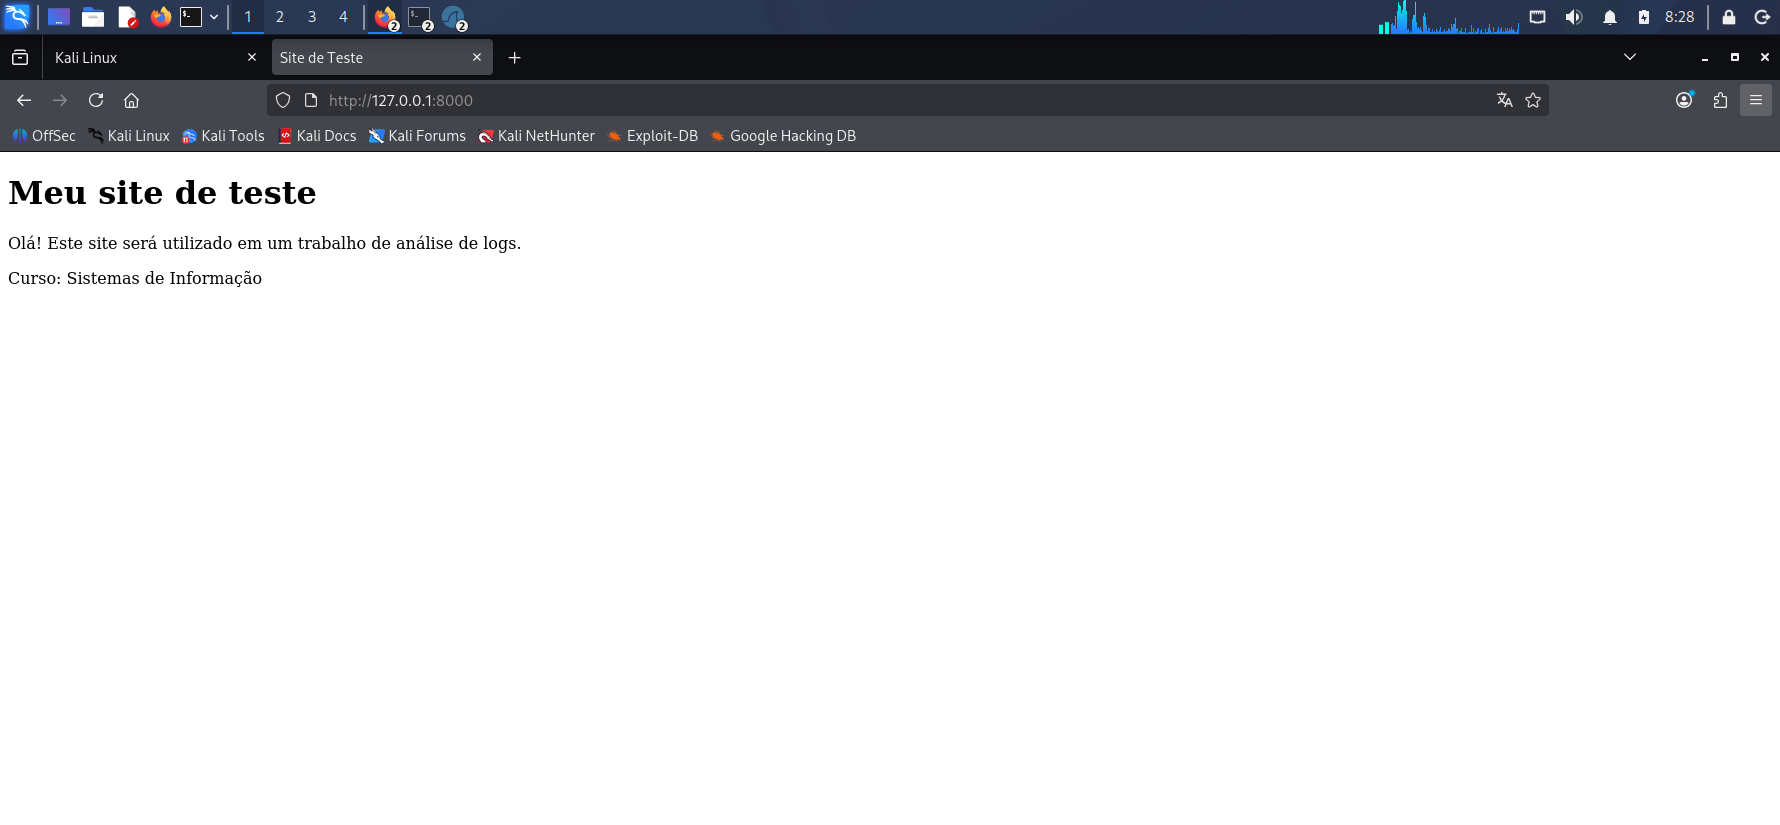
\includegraphics[width=.48\textwidth]{img/fig1-pagina-teste.png}
\caption{Página HTML de teste acessada pelo servidor HTTP local na porta 8000.}
\label{fig:pagina-teste}
\end{figure}

Com o Wireshark capturando a interface \texttt{lo}, cada atualização da
página no navegador gerou uma nova sequência de pacotes TCP e HTTP, na
qual é possível identificar o padrão típico de uma transação HTTP curta:
os segmentos do \textit{three-way handshake}, o pacote contendo a
requisição \texttt{GET}, o pacote de resposta do servidor e, por fim, os
segmentos de encerramento da conexão.

\FloatBarrier
\subsection{Estabelecimento da conexão TCP}

Antes da troca de mensagens HTTP, o Wireshark permitiu identificar os três
pacotes responsáveis pelo estabelecimento da conexão TCP, conhecido como
\textit{Three-Way Handshake} \cite{postel1981}: um segmento \texttt{SYN}
enviado pelo cliente a partir de uma porta temporária em direção à porta
8000 do servidor; um segmento \texttt{SYN, ACK} enviado pelo servidor em
resposta; e um segmento \texttt{ACK} enviado pelo cliente, que finaliza o
handshake (Figura~\ref{fig:handshake}). Esses três segmentos apresentam
comprimento de dados (\textit{TCP Segment Len}) igual a zero, pois sua
função é apenas estabelecer a conexão, e não transportar conteúdo da
aplicação. Somente após essa etapa é enviada a requisição HTTP GET.

\begin{figure}[ht]
\centering
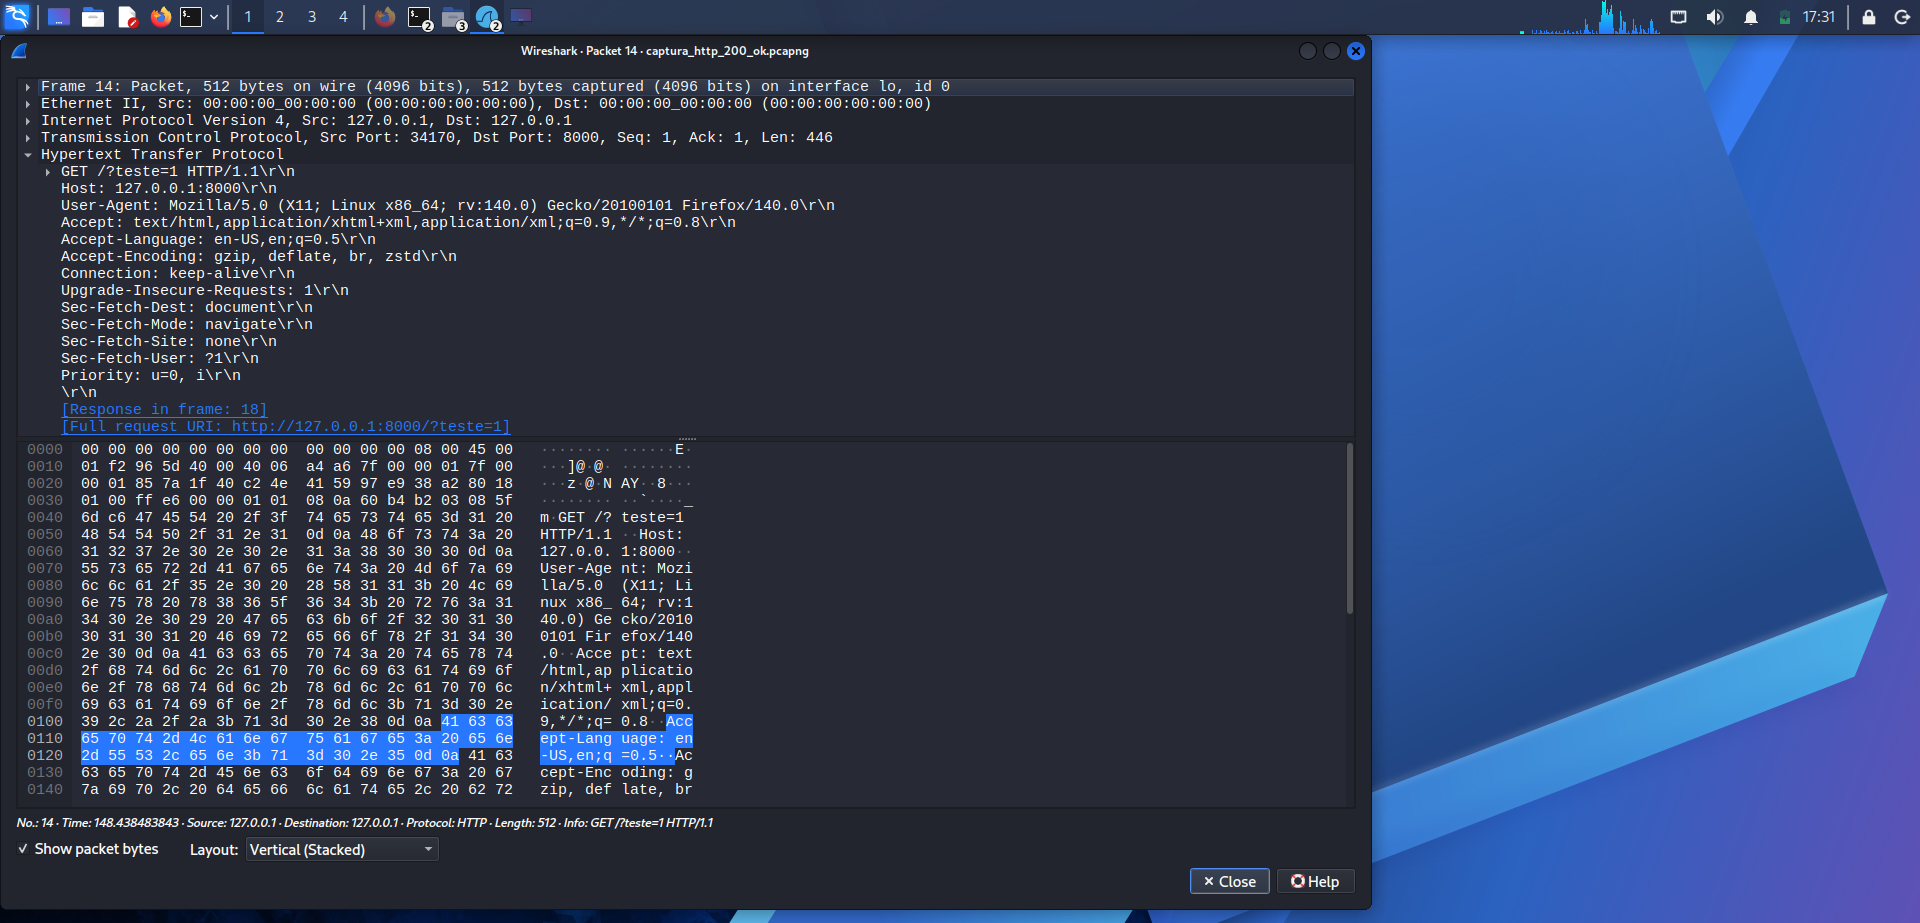
\includegraphics[width=.50\textwidth]{img/fig6-handshake-tcp.png}
\caption{Detalhe de um dos segmentos do estabelecimento da conexão TCP
  (\textit{Three-Way Handshake}), com a flag ACK confirmada.}
\label{fig:handshake}
\end{figure}

\FloatBarrier
\subsection{Requisição HTTP GET}

Após o handshake, o pacote seguinte contém a requisição HTTP realizada
pelo navegador. A Figura~\ref{fig:get} mostra o detalhe de uma dessas
requisições, na qual se observa a linha inicial \texttt{GET / HTTP/1.1},
o campo \texttt{Host}, identificando o servidor de destino
(\texttt{127.0.0.1:8000}), e o campo \texttt{User-Agent}, contendo
informações sobre o navegador utilizado.

\begin{figure}[ht]
\centering
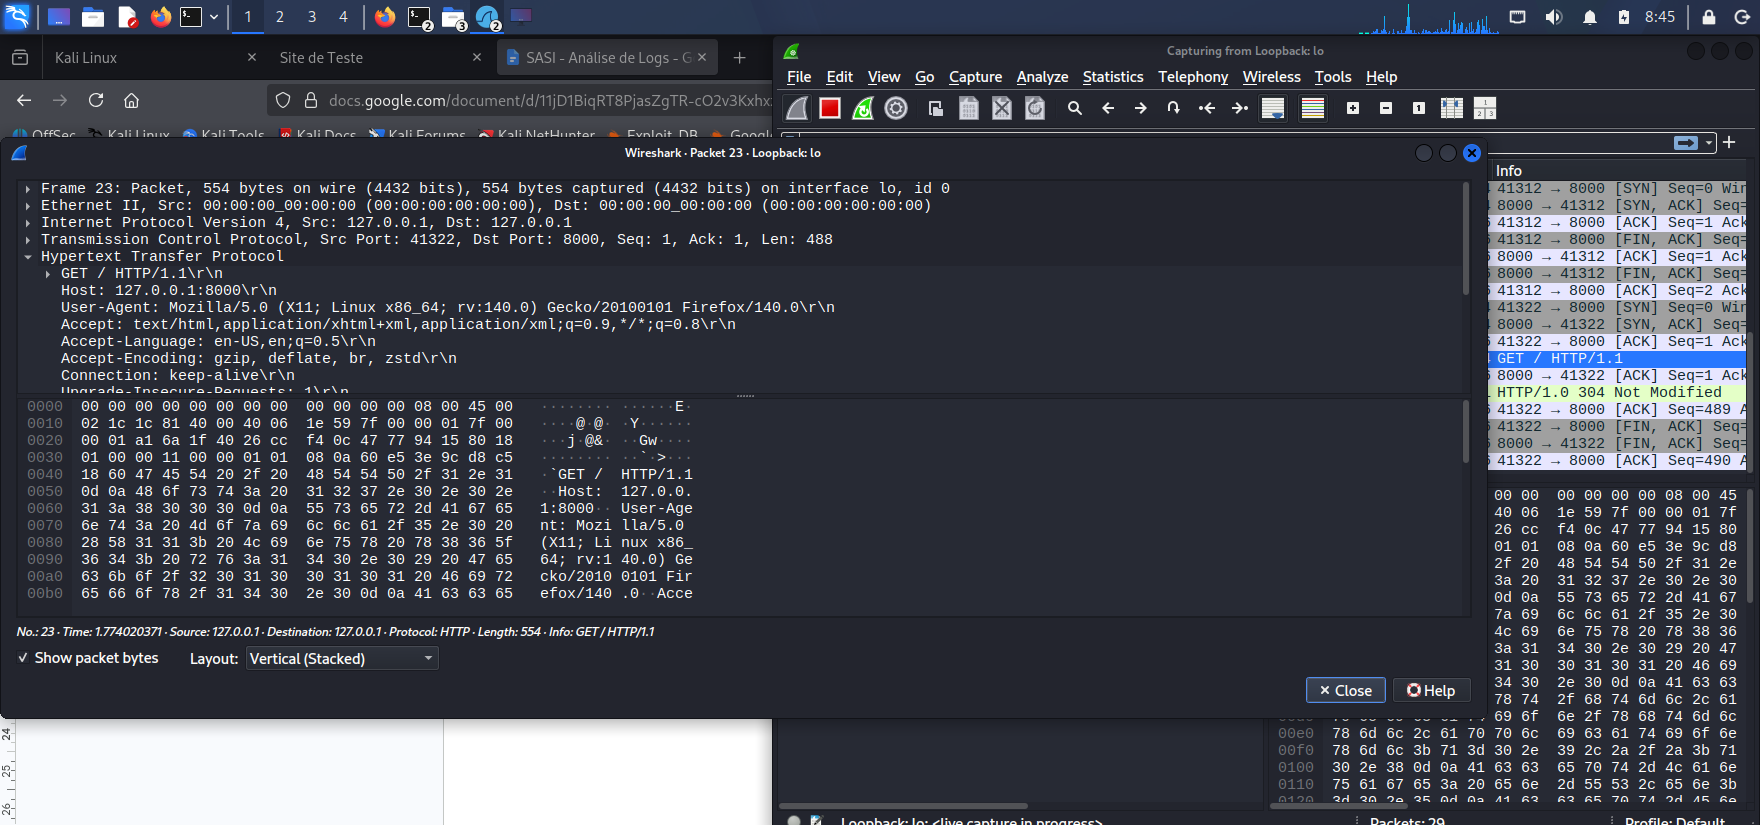
\includegraphics[width=.50\textwidth]{img/fig3-requisicao-get.png}
\caption{Requisição HTTP GET capturada pelo Wireshark durante o acesso ao servidor.}
\label{fig:get}
\end{figure}

Uma análise mais detalhada dos cabeçalhos da requisição, apresentada na
Figura~\ref{fig:headers}, revela ainda os campos \texttt{Accept},
\texttt{Accept-Language} e \texttt{Accept-Encoding}, que informam,
respectivamente, os tipos de conteúdo, os idiomas e os métodos de
compressão aceitos pelo cliente, além do campo \texttt{Connection:
keep-alive}, relacionado à manutenção da conexão para requisições
subsequentes. O Wireshark também relaciona automaticamente a requisição à
sua resposta por meio da anotação \texttt{[Response in frame: N]}, o que
facilita seguir o fluxo completo da transação.

\begin{figure}[ht]
\centering
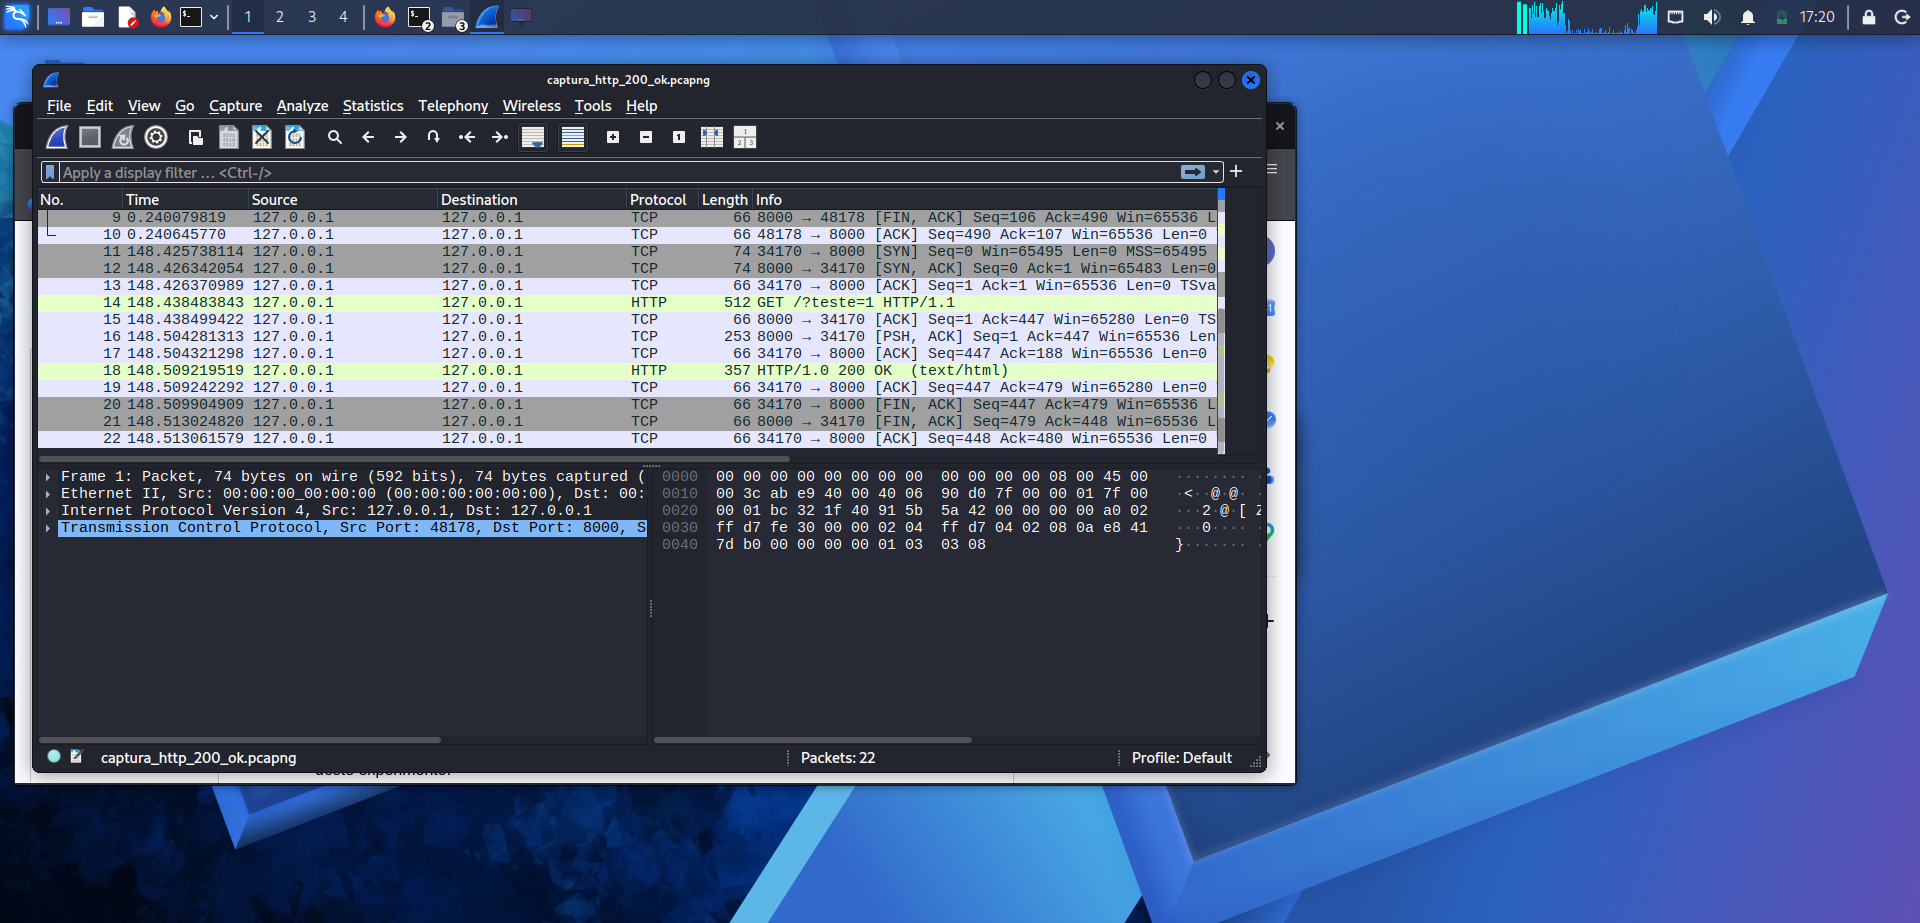
\includegraphics[width=.50\textwidth]{img/fig5-cabecalhos-requisicao.png}
\caption{Cabeçalhos completos de uma requisição HTTP GET, incluindo campos
  \texttt{Accept}, \texttt{Accept-Language} e \texttt{Connection}.}
\label{fig:headers}
\end{figure}

Do ponto de vista da segurança, esse resultado já demonstra que uma
requisição HTTP revela, a qualquer observador com acesso ao tráfego,
informações sobre o recurso solicitado e sobre o cliente que o solicitou.

\FloatBarrier
\subsection{Respostas do servidor: 304 e 200 OK}

Duas situações de resposta foram observadas no experimento. Na primeira
requisição, o servidor respondeu com o código \texttt{304 Not Modified},
indicando que o recurso solicitado não havia sido alterado desde o último
acesso e que o navegador poderia utilizar a versão já armazenada em cache,
sem a necessidade de reenviar todo o conteúdo. Para obter uma nova
transferência de conteúdo, uma segunda requisição foi realizada utilizando
o parâmetro \texttt{?teste=1}, o que tornou a URL diferente da anterior e
evitou o uso do cache pelo navegador.

Essa segunda requisição resultou em uma resposta \texttt{HTTP/1.0 200 OK}
(Figura~\ref{fig:ok}), na qual foram identificados campos relevantes:
\texttt{Server: SimpleHTTP/0.6 Python/3.13.12}, identificando o software do
servidor; \texttt{Content-Type: text/html}, indicando o tipo do conteúdo
enviado; e \texttt{Content-Length}, informando o tamanho da resposta em
bytes. O Wireshark relaciona ainda essa resposta à requisição
correspondente por meio da anotação \texttt{[Request in frame: N]}.

\begin{figure}[ht]
\centering
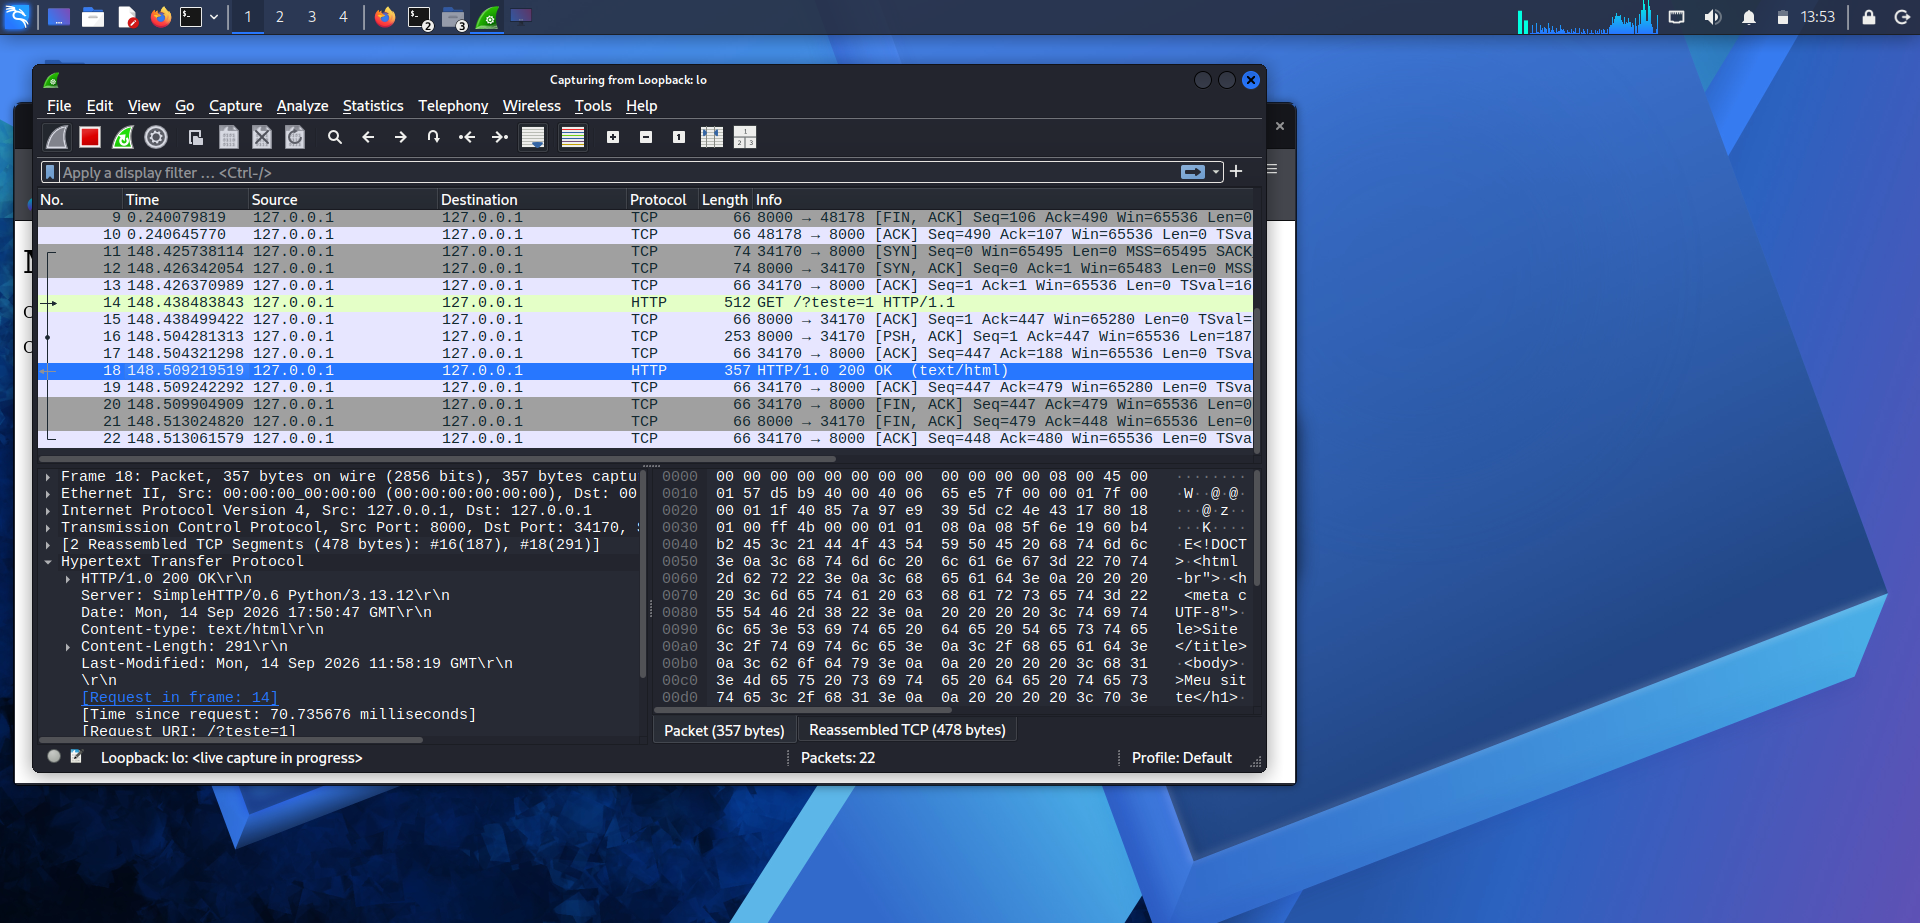
\includegraphics[width=.50\textwidth]{img/fig4-resposta-200-ok.png}
\caption{Resposta HTTP/1.0 200 OK, contendo os cabeçalhos do servidor e o
  início do conteúdo HTML (\texttt{<!DOCTYPE html>}) em texto claro.}
\label{fig:ok}
\end{figure}

\FloatBarrier
\subsection{Visualização do conteúdo transmitido}

Ainda na resposta \texttt{200 OK}, foi possível observar, diretamente nos
dados do pacote, o conteúdo HTML transmitido pelo servidor, incluindo
trechos como \texttt{<title>Site de Teste</title>}, \texttt{<h1>Meu site de
teste</h1>} e \texttt{<p>Curso: Sistemas de Informação</p>}. Isso ocorre
porque a comunicação analisada utiliza HTTP sem criptografia: o conteúdo
transmitido pode ser observado em texto legível por qualquer ferramenta
que tenha acesso ao tráfego, como demonstrado neste experimento controlado.
Em comunicações HTTPS, por outro lado, o conteúdo da camada de aplicação é
protegido por criptografia durante o transporte, graças ao uso do TLS
\cite{rescorla2018}.

\FloatBarrier
\subsection{Encerramento da conexão TCP}

Após a troca das mensagens HTTP, foi analisado também o encerramento da
conexão TCP. Foi identificado um segmento com as \textit{flags}
\texttt{FIN} e \texttt{ACK} simultaneamente ativas (\texttt{Flags: 0x011}),
enviado pela porta temporária do cliente em direção à porta 8000 do
servidor (Figura~\ref{fig:fin}). A flag \texttt{FIN} indica a intenção de
finalizar o envio de dados em uma direção da conexão, enquanto a flag
\texttt{ACK} confirma o recebimento de informações anteriores. O segmento
apresentou \textit{TCP Segment Len} igual a zero, confirmando que se
tratava de um segmento de controle, sem dados de aplicação.

\begin{figure}[ht]
\centering
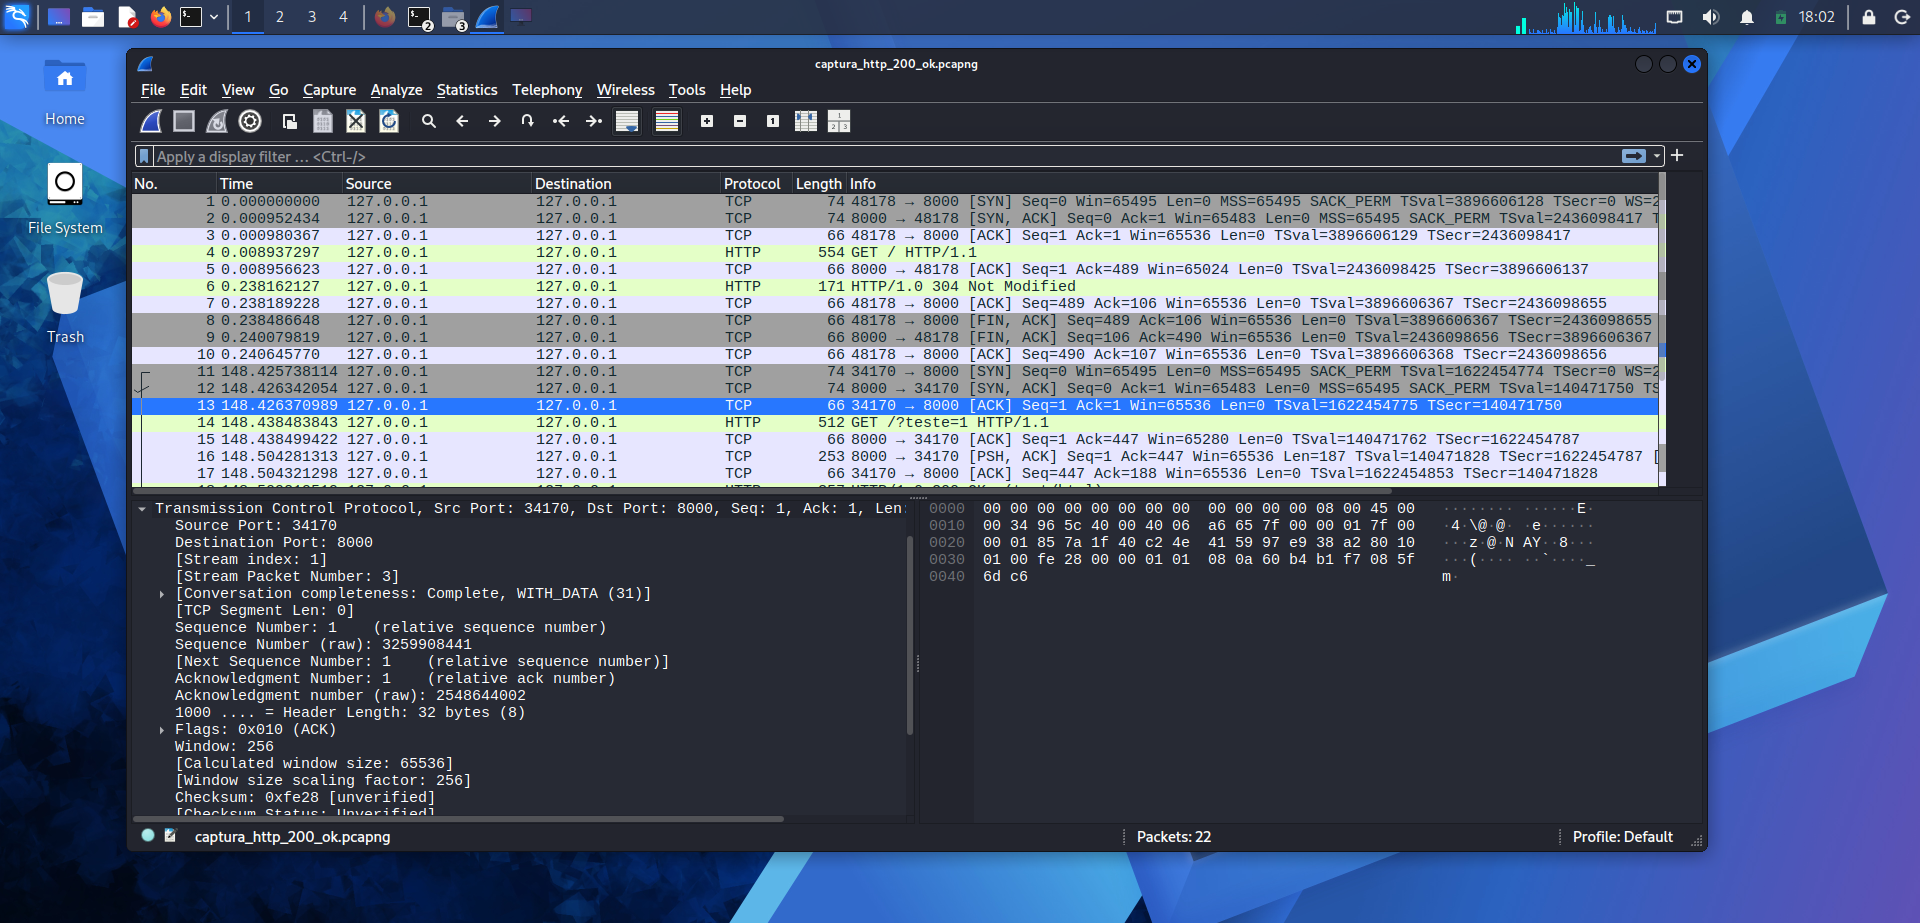
\includegraphics[width=.50\textwidth]{img/fig7-encerramento-tcp.png}
\caption{Segmento TCP com as flags FIN e ACK ativas, utilizado no
  encerramento da conexão.}
\label{fig:fin}
\end{figure}

Esse resultado evidencia que o TCP participa tanto do estabelecimento
quanto do encerramento da comunicação utilizada pelo HTTP, de modo que o
Wireshark permitiu acompanhar não apenas as mensagens HTTP, mas também as
etapas da camada de transporte responsáveis por viabilizar essa
comunicação.

\FloatBarrier
\subsection{Reconstrução da comunicação com Follow HTTP Stream}

Como etapa final da análise, foi utilizada a funcionalidade
\textit{Follow HTTP Stream} do Wireshark, que reúne, em uma única
visualização, todos os dados pertencentes ao mesmo fluxo de comunicação
entre cliente e servidor. A Figura~\ref{fig:stream} mostra essa
reconstrução, na qual é possível observar, em sequência, a requisição
completa enviada pelo navegador (método, \texttt{Host} e demais
cabeçalhos) e a resposta completa do servidor (linha de status,
cabeçalhos e conteúdo HTML).

\begin{figure}[ht]
\centering
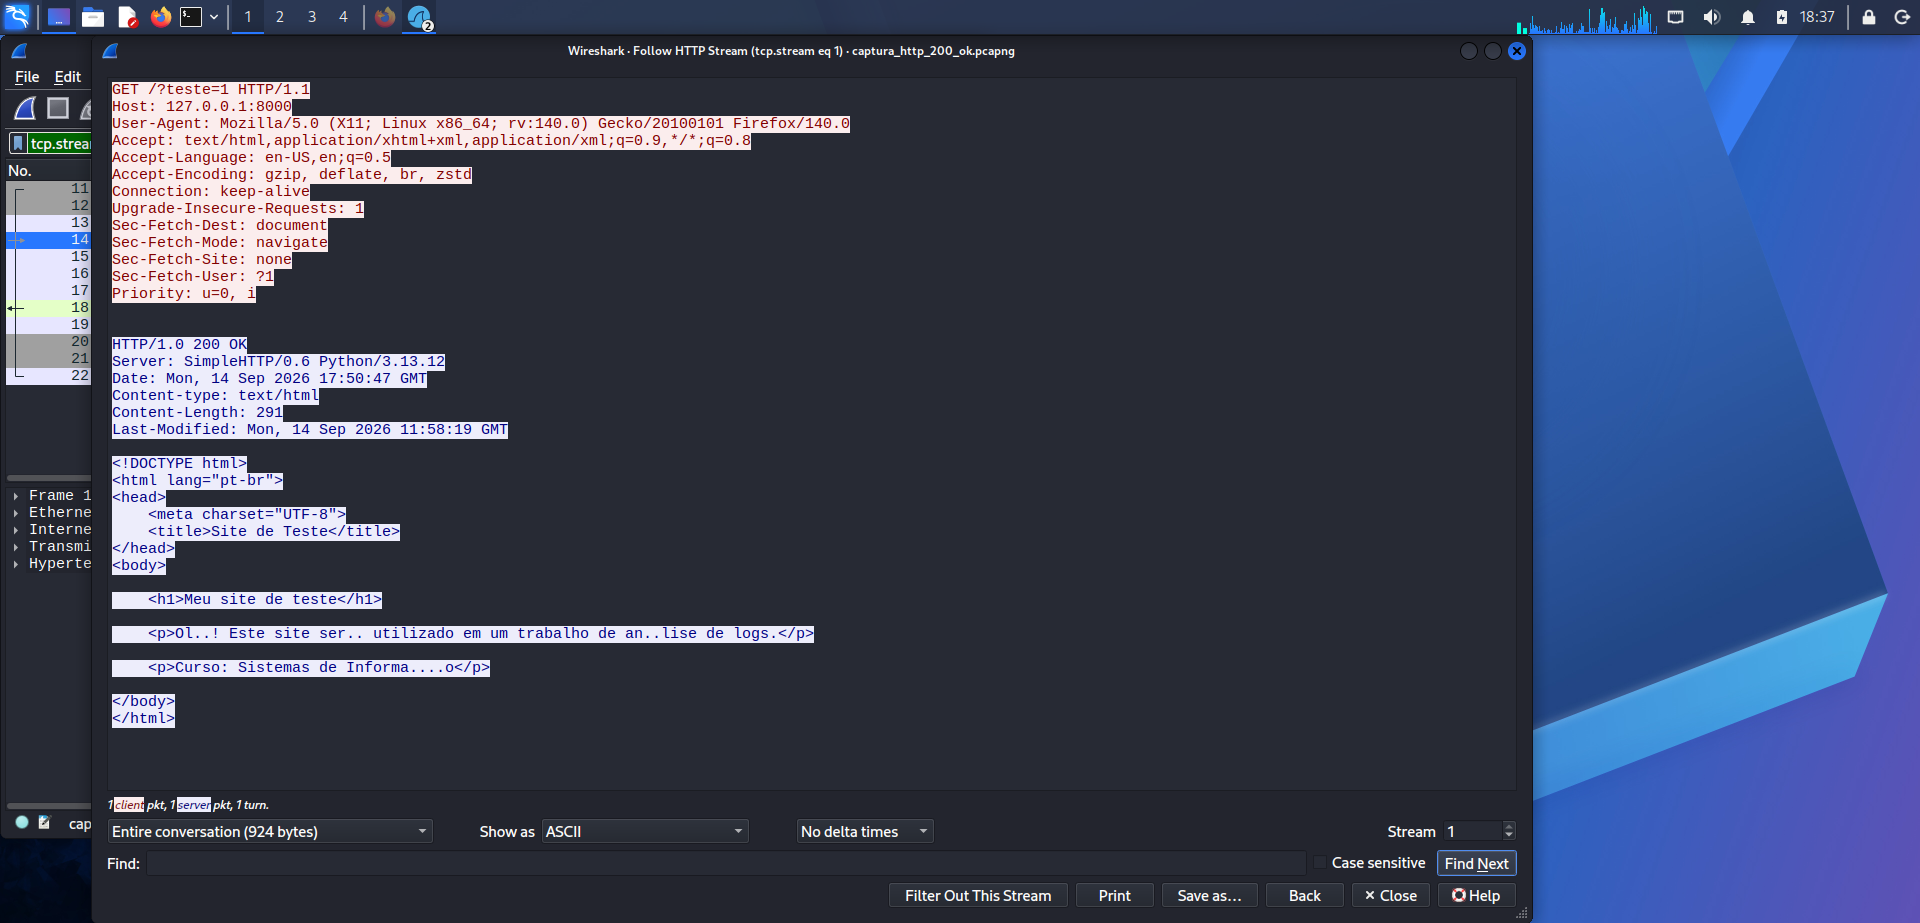
\includegraphics[width=.50\textwidth]{img/fig8-follow-http-stream.png}
\caption{Reconstrução do fluxo HTTP completo utilizando a funcionalidade
  Follow HTTP Stream do Wireshark.}
\label{fig:stream}
\end{figure}

Essa visualização resume o principal resultado deste primeiro experimento
do ponto de vista da segurança: em uma comunicação HTTP sem criptografia,
tanto os metadados quanto o conteúdo da camada de aplicação podem ser
inspecionados em texto legível por qualquer observador com acesso ao
tráfego de rede \cite{stallings2015,kurose2021}.

\FloatBarrier
\subsection{Contraste com HTTPS: tráfego cifrado}

No segundo experimento, a mesma interface de loopback foi capturada durante
a sequência de login e consulta de perfil na API HTTPS. Ao contrário do
primeiro experimento, a lista de pacotes não mostra nenhuma requisição ou
resposta HTTP em texto claro: após o \textit{handshake} TCP, o Wireshark
identifica apenas as etapas do TLS 1.3 (\texttt{Client Hello},
\texttt{Server Hello, Change Cipher Spec}) e, em seguida, pacotes rotulados
apenas como \texttt{Application Data} (Figura~\ref{fig:tls-appdata}), cujo
painel de bytes mostra dados sem estrutura reconhecível -- nenhum vestígio
da URL, do login ou do token.

\begin{figure}[ht]
\centering
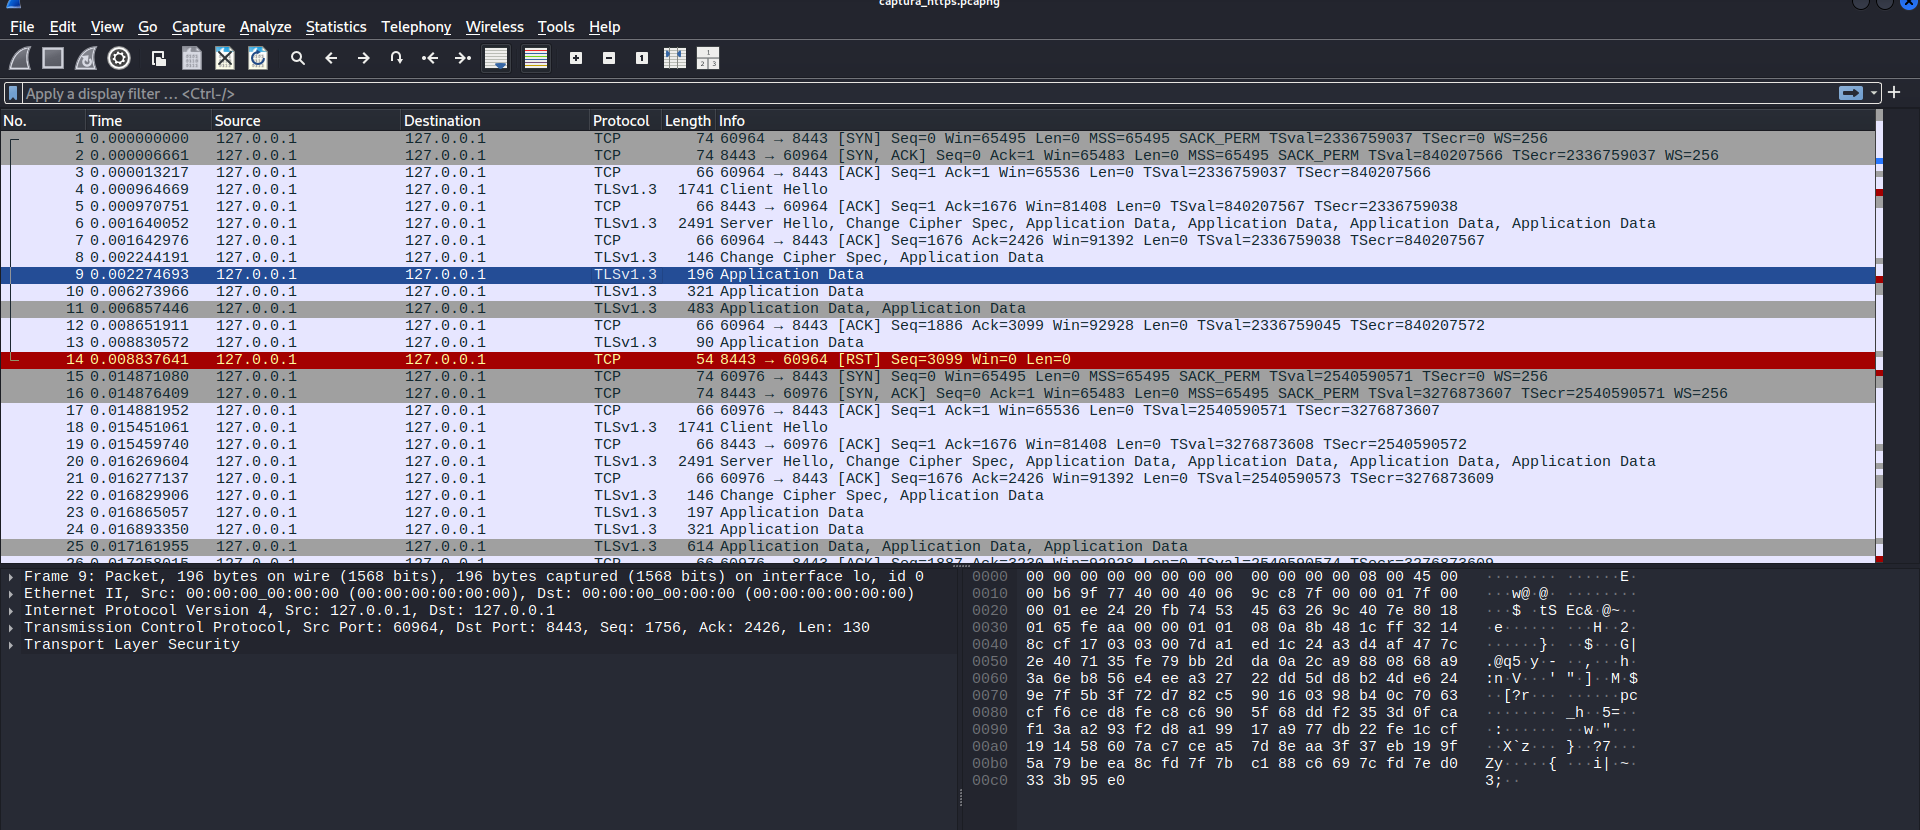
\includegraphics[width=.50\textwidth]{img/fig9-https-application-data.png}
\caption{Captura da mesma comunicação em HTTPS: após o handshake TLS, o
  Wireshark só identifica pacotes de \texttt{Application Data} cifrados,
  sem conteúdo legível no painel de bytes.}
\label{fig:tls-appdata}
\end{figure}

Esse resultado confirma, na prática, o papel do TLS descrito na
Seção~\ref{sec:metodo}: diferentemente do que ocorreu com o servidor HTTP
puro, aqui não é possível recuperar credenciais, tokens ou dados de
resposta a partir da captura de pacotes, mesmo utilizando a mesma
ferramenta e a mesma interface de rede.

\FloatBarrier
\subsection{Falha de autorização entre objetos (BOLA) em uma API HTTPS}

Embora a captura de rede não revele mais o conteúdo das mensagens, a
cadeia de requisições executada contra a própria API expõe uma falha que a
criptografia de transporte não é capaz de corrigir. A
Figura~\ref{fig:bola-terminal} mostra a execução completa do
procedimento descrito na Seção~\ref{sec:metodo}.

\begin{figure}[ht]
\centering
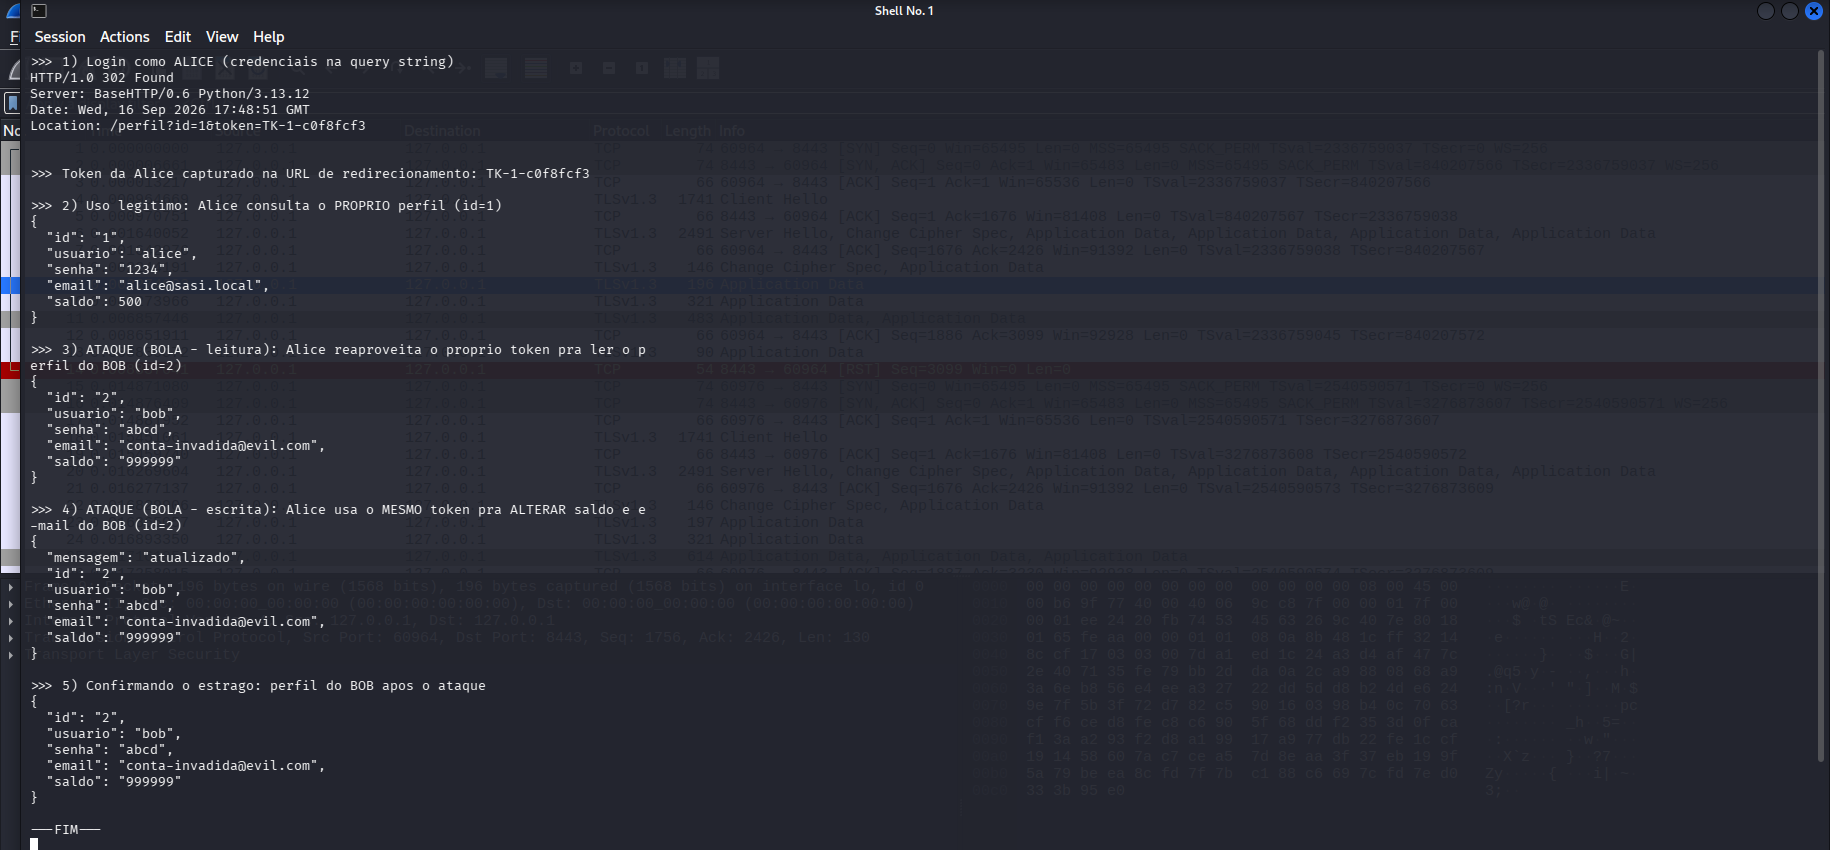
\includegraphics[width=.50\textwidth]{img/fig10-exploit-bola-terminal.png}
\caption{Execução da cadeia de exploração da falha BOLA: login como
  \texttt{alice}, consulta ao próprio perfil, leitura indevida e alteração
  dos dados de \texttt{bob} reaproveitando o token de \texttt{alice}.}
\label{fig:bola-terminal}
\end{figure}

O login como \texttt{alice} devolve o token na própria URL de
redirecionamento (\texttt{Location: /perfil?id=1\&token=TK-1-c0f8fcf3}) --
já uma prática desaconselhada, pois URLs completas tendem a ficar
registradas em históricos de navegador, logs de servidor e
\textit{proxies}, independentemente do uso de HTTPS \cite{fielding2014}.
O passo seguinte usa esse token corretamente, com \texttt{id=1}, e retorna
os dados da própria \texttt{alice}.

O problema aparece ao trocar apenas o parâmetro para \texttt{id=2} --
mantendo o token de \texttt{alice} --: a API devolve integralmente o
perfil de \texttt{bob}. Isso ocorre porque a rota \texttt{/perfil} verifica
somente se o token \textit{existe}, sem checar se ele pertence ao
\texttt{id} solicitado -- exatamente a definição de BOLA (API1:2023 do
OWASP API Security Top 10) \cite{owasp-api2023}. Em seguida, a mesma falha
é explorada por escrita: um \texttt{POST} para \texttt{/perfil/atualizar},
ainda com o token de \texttt{alice} mas \texttt{id=2}, altera o e-mail de
\texttt{bob} para \texttt{conta-invadida@evil.com} e seu saldo para
\texttt{999999}, sem que as credenciais de \texttt{bob} jamais tivessem
sido comprometidas -- o ataque depende apenas de um token válido de
\emph{qualquer} usuário autenticado.

Esse resultado ilustra um ponto central para a auditoria de segurança de
APIs: HTTPS é necessário, mas não suficiente. Ele impede que um observador
de rede leia credenciais e tokens em trânsito, mas não substitui a
validação, a cada requisição, de que o dono do token tem permissão sobre o
objeto acessado ou modificado.

\FloatBarrier
\section{Conclusão}\label{sec:conclusao}

Este trabalho utilizou o Wireshark em dois experimentos complementares. No
primeiro, a captura de uma comunicação HTTP sem criptografia permitiu
identificar o \textit{Three-Way Handshake}, a requisição GET, os
cabeçalhos, as respostas \texttt{304}/\texttt{200 OK}, o conteúdo HTML
transmitido e o encerramento da conexão -- tudo em texto legível
diretamente no Wireshark, sem qualquer esforço adicional de decodificação.

O segundo experimento mostrou que essa não é toda a história. Ao repetir a
captura contra uma API HTTPS, o Wireshark deixou de conseguir ler qualquer
credencial, token ou conteúdo de resposta, confirmando que o TLS cumpre seu
papel de proteger os dados em trânsito. Mesmo assim, a mesma API se mostrou
vulnerável a uma falha de autorização entre objetos (BOLA): por não
verificar se o token de sessão pertencia ao usuário solicitado, ela
permitiu ler e alterar dados de outro usuário apenas manipulando um
parâmetro na requisição, sem nunca comprometer credenciais alheias. Isso
evidencia, na prática, que HTTPS e controle de acesso adequado são medidas
complementares: criptografia de transporte protege a confidencialidade na
rede, mas só uma verificação correta de autorização no servidor evita que
falhas de lógica de aplicação sejam exploradas por usuários autenticados
mal-intencionados.

Como trabalho futuro, sugere-se corrigir a API, verificando se o
\texttt{id} do objeto corresponde ao dono do token, e repetir os testes
para confirmar que o ataque deixa de funcionar.

{\small
\bibliographystyle{sbc}
\bibliography{referencias}
}

\end{document}
